%\documentclass{article}
%\usepackage{graphicx,subfigure}
%\begin{document}

\begin{figure}[h]
  \centering
  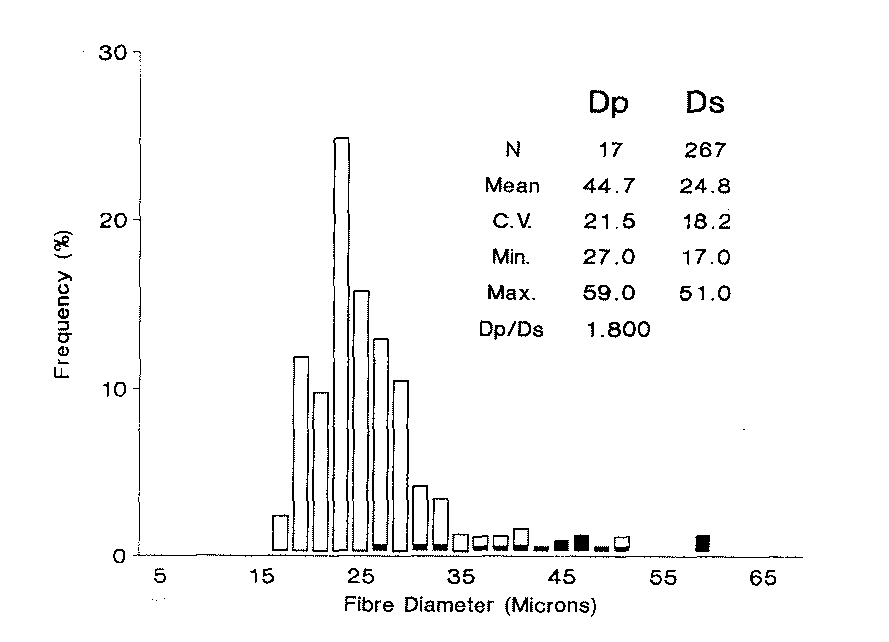
\includegraphics[width=\textwidth,trim = 0 0 0 20]{images/fig13ri.png}
  \caption{Fibre diameter histogram of a 198? drop hogget ewe from CSIRO
      experiment No. 10.  Note the high frequency of large primary and
      secondary fibres.}
  \label{fig:13}
\end{figure}

%\end{document}
